%!TEX root=../Thesis.tex
\begin{figure}[ht]
\centering
\begin{subfigure}[b]{0.45\textwidth}
    \centering
    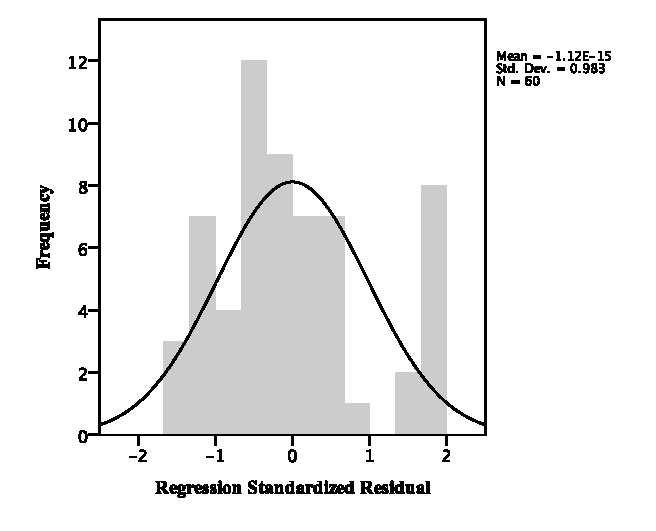
\includegraphics[width=\textwidth]{images/normality/ValMax/HistValMax.eps}
    \caption{Histogram}
    \label{fig:histvalmax}
\end{subfigure}
\quad
\begin{subfigure}[b]{0.45\textwidth}
    \centering
    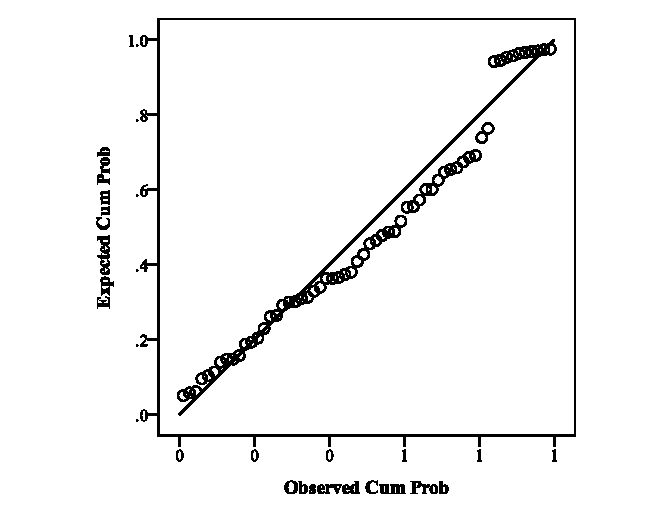
\includegraphics[width=\textwidth]{images/normality/ValMax/PPValMax.eps}
    \caption{P-P plot}
    \label{fig:ppvalmax}
\end{subfigure}
\caption{Normality graphs for valence, maximum tap pressure and duration.}
\end{figure}
\par\bigskip
\par\bigskip
\begin{figure}[ht]
\centering
\begin{subfigure}[b]{0.45\textwidth}
    \centering
    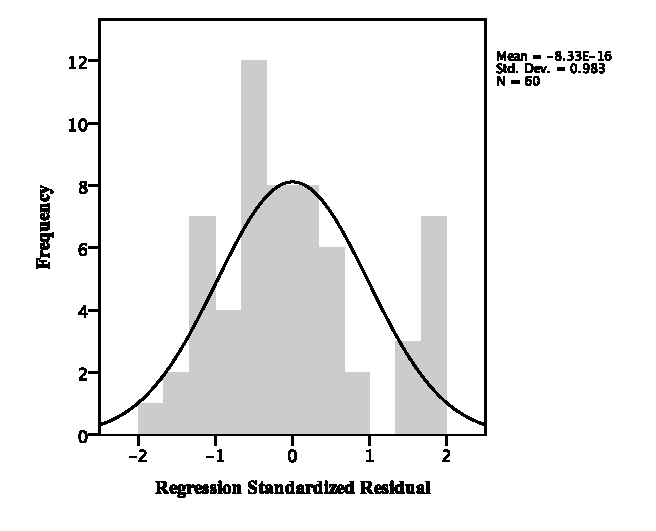
\includegraphics[width=\textwidth]{images/normality/valavg/HistValAvg.eps}
    \caption{Histogram}
    \label{fig:histvalavg}
\end{subfigure}
\quad
\begin{subfigure}[b]{0.45\textwidth}
    \centering
    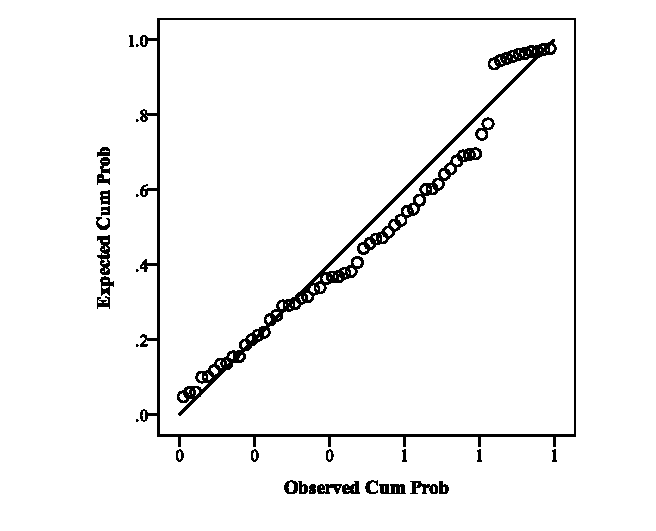
\includegraphics[width=\textwidth]{images/normality/valavg/PPValAvg.eps}
    \caption{P-P plot}
    \label{fig:ppvalavg}
\end{subfigure}
\caption{Normality graphs for valence, average tap pressure and duration.}
\end{figure}
\par\bigskip
\par\bigskip
\begin{figure}[ht]
\centering
\begin{subfigure}[b]{0.45\textwidth}
    \centering
    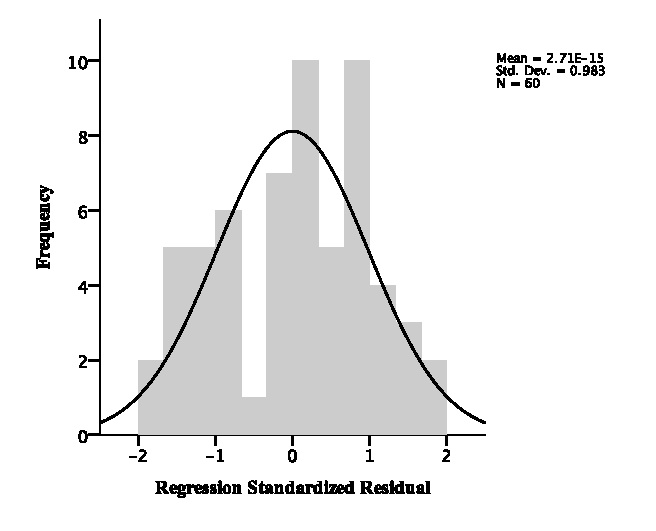
\includegraphics[width=\textwidth]{images/normality/ArMax/HistArMax.eps}
    \caption{Histogram}
    \label{fig:histarmax}
\end{subfigure}
\quad
\begin{subfigure}[b]{0.45\textwidth}
    \centering
    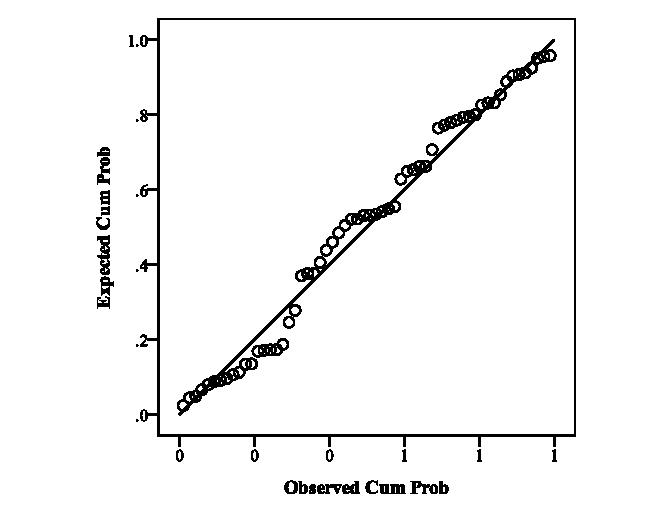
\includegraphics[width=\textwidth]{images/normality/ArMax/PPArMax.eps}
    \caption{P-P plot}
    \label{fig:pparmax}
\end{subfigure}
\caption{Normality graphs for arousal, average tap pressure and duration.}
\end{figure}
\par\bigskip
\par\bigskip
\begin{figure}[ht]
\centering
\begin{subfigure}[b]{0.45\textwidth}
    \centering
    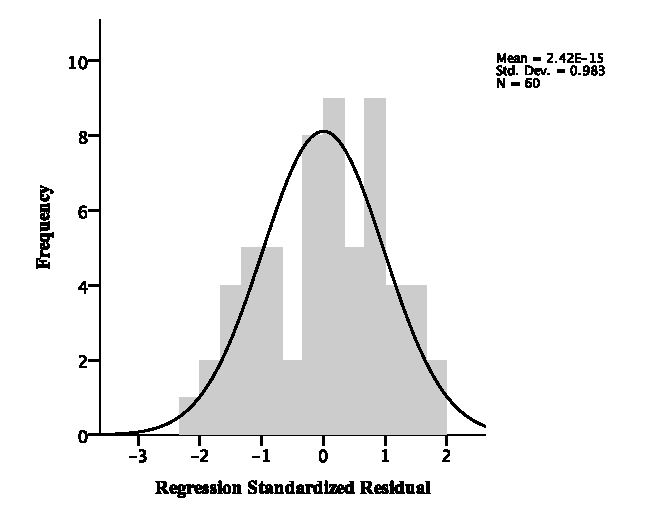
\includegraphics[width=\textwidth]{images/normality/aravg/HistArAvg.eps}
    \caption{Histogram}
    \label{fig:histaravg}
\end{subfigure}
\quad
\begin{subfigure}[b]{0.45\textwidth}
    \centering
    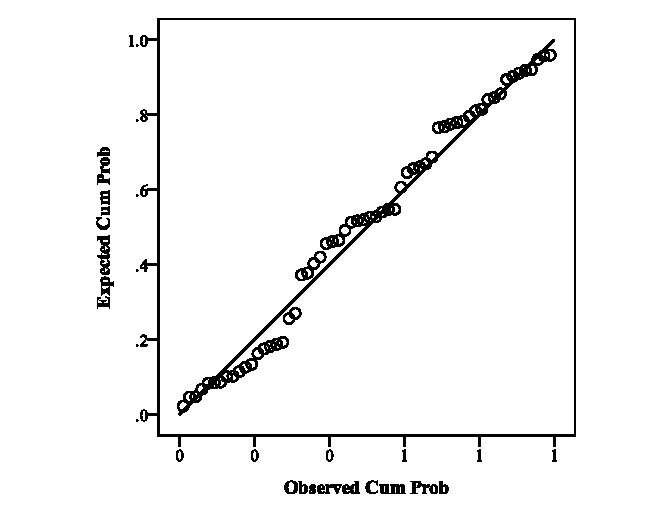
\includegraphics[width=\textwidth]{images/normality/aravg/PPArAvg.eps}
    \caption{P-P plot}
    \label{fig:pparavg}
\end{subfigure}
\caption{Normality graphs for arousal, average tap pressure and duration.}
\end{figure}